\chapter{Neural Network Fundamentals}
\label{ch:lesson31}

Chapter~\ref{ch:lesson30} hand-picked a projection direction $w$ (the difference of class means) to separate two classes. That worked, but it required a human to notice a good heuristic. This chapter replaces the human with \textbf{gradient descent}: an automatic procedure that \emph{learns} $w$ and $b$ directly from data by repeatedly nudging them to reduce a loss. The recipe --- forward pass, loss, backward pass, update --- is the entire training loop behind every neural network in this course, no matter how large.

\section{A new library: PyTorch and tensors}

From here on, most chapters lean on \textbf{PyTorch} rather than OpenCV, because training neural networks needs two things OpenCV was never designed for: automatic differentiation (computing gradients of arbitrarily complex functions) and GPU acceleration for large matrix multiplications. A \textbf{tensor} is simply the general term for a grid of numbers of any dimensionality --- every array used so far in this course has really been a tensor all along; PyTorch's \code{torch.Tensor} is NumPy's \code{ndarray} with two extras: it can track a \code{.grad} for automatic differentiation, and it can live on a GPU.

Two PyTorch conventions worth flagging up front: it stores color images \textbf{channel-first}, as \code{(channel, height, width)} rather than NumPy/OpenCV's \code{(height, width, channel)} from Chapter~\ref{ch:lesson01}; and its layers almost always expect a \textbf{batch dimension} first, even for a single example.

\section{A binary classification problem}

We reuse the same two-class dataset from Chapter~\ref{ch:lesson30} (Figure~\ref{fig:l31-1}), so the learned direction below can be compared directly against the hand-picked one.

\begin{figure}[h]
\centering
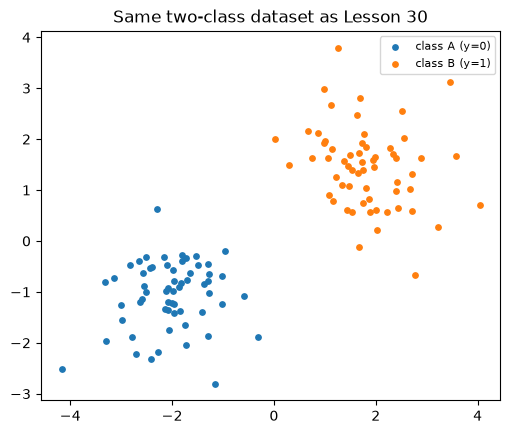
\includegraphics[width=0.6\textwidth]{figures/lesson31_fig01.png}
\caption{The same two-class dataset from Chapter~\ref{ch:lesson30}.}
\label{fig:l31-1}
\end{figure}

\section{From a raw score to a probability}

Recall the projection from Chapter~\ref{ch:lesson30}: a single neuron computes a raw score $z=w^\top x+b$, then classifies by that score's sign. The goal of training is to find a $w$ and $b$ that make $z$ come out positive for class B and negative for class A --- but instead of hand-picking them, gradient descent should find them automatically.

The trouble is that classification accuracy (right or wrong) is flat almost everywhere and jumps discontinuously at the decision boundary --- it has no useful gradient to follow. The fix: squash the raw score through the \textbf{sigmoid} function, which maps any real number to a smooth value between 0 and 1, read as ``how confident is the model that this point is class B?''
\begin{equation}
\sigma(z) = \frac{1}{1+e^{-z}}.
\end{equation}
A large positive $z$ maps close to 1, a large negative $z$ close to 0, and $z=0$ maps to exactly 0.5, right on the fence (Figure~\ref{fig:l31-2}).

\begin{figure}[h]
\centering
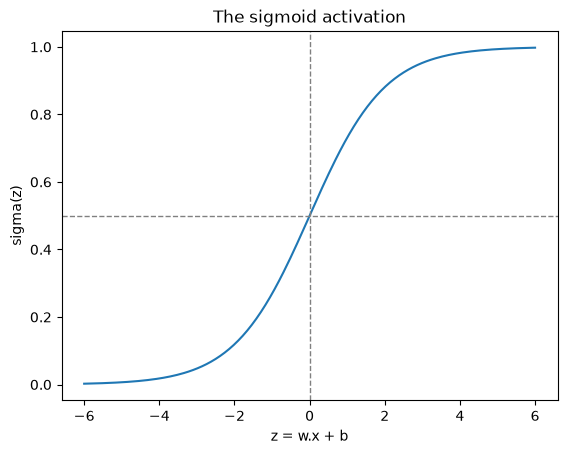
\includegraphics[width=0.55\textwidth]{figures/lesson31_fig02.png}
\caption{The sigmoid activation.}
\label{fig:l31-2}
\end{figure}

\section{Binary cross-entropy: turning probability into a trainable loss}

A probability alone isn't yet something to optimize. Training needs a single number --- \textbf{loss} --- that's small when the model's probabilities are good and large when they're bad. \textbf{Binary cross-entropy} penalizes each prediction according to how confident it was, and whether that confidence was justified: if the true label is 1, the penalty is $-\log(p)$ (near zero when $p$ is close to 1, exploding as $p\to0$); if the true label is 0, the mirror image, $-\log(1-p)$ (Figure~\ref{fig:l31-3}).

\begin{figure}[h]
\centering
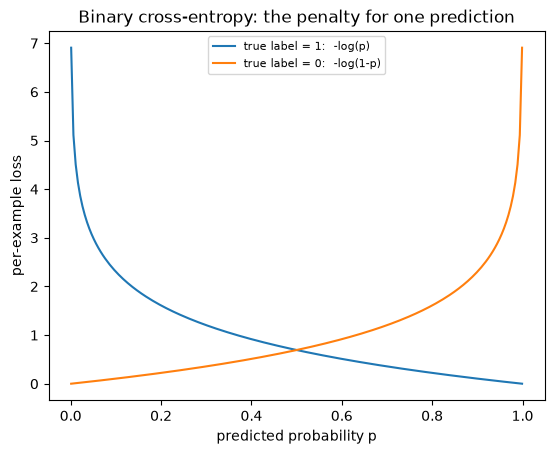
\includegraphics[width=0.6\textwidth]{figures/lesson31_fig03.png}
\caption{Binary cross-entropy: the penalty for one prediction, as a function of the predicted probability.}
\label{fig:l31-3}
\end{figure}

Averaging that per-example penalty over the whole dataset gives the full loss:
\begin{equation}
L = -\frac{1}{n}\sum_i\big[y_i\log\sigma(z_i) + (1-y_i)\log(1-\sigma(z_i))\big].
\end{equation}
This is exactly the two curves above, selected by $y_i$ (only one term is ever nonzero, since $y_i$ is 0 or 1) and averaged over every point. Because both the sigmoid and the logarithm are smooth, $L$ has a well-defined gradient everywhere --- the loss decreases smoothly as predictions get closer to being correct, instead of only changing at the decision boundary.

\section{Backpropagation: the chain rule, applied}

``Backprop'' is just the chain rule from Chapters~\ref{ch:lesson12}--\ref{ch:lesson13}, applied to a composed function: $L$ depends on $\sigma(z)$, which depends on $z=w^\top x+b$, which depends on $w$ and $b$. Working backward through that chain (skipping the algebra) gives a remarkably clean result:
\begin{equation}
\frac{\partial L}{\partial z_i} = \sigma(z_i) - y_i, \qquad \frac{\partial L}{\partial w} = \frac{1}{n}X^\top(\sigma(z)-y), \qquad \frac{\partial L}{\partial b} = \frac{1}{n}\sum_i(\sigma(z_i)-y_i).
\end{equation}
In words: the gradient is just the \emph{prediction error}, averaged (weighted by $x$ for $w$'s gradient). Wildly wrong predictions push the weights hard; correct ones barely move them at all.

\subsection*{Sanity checks: numerical gradient and PyTorch autograd}

Before trusting any hand-derived gradient, it's standard practice to check it two independent ways. First, numerically: perturb each parameter by a tiny amount and see how much the loss actually changes, compared to the analytical formula --- the finite-difference and analytic gradients agree to a max discrepancy of $1.01\times10^{-9}$. Second, via PyTorch's automatic differentiation (\code{.backward()}, using its built-in \code{binary\_cross\_entropy\_with\_logits}) --- agreeing with the hand-derived gradient to $5.55\times10^{-17}$. This kind of double-checking is standard practice whenever a gradient is derived by hand.

\section{Training: the full loop}

Initialize $w,b$ randomly (not with a clever heuristic this time), then repeat: forward pass, compute loss, backward pass, take a small step \emph{against} the gradient (gradient \emph{descent}, since the gradient points toward increasing loss).

\begin{lstlisting}
def train(X, y, n_epochs=500, lr=0.5, seed=0):
    w = rng.normal(size=X.shape[1]) * 0.1
    b = 0.0
    for _ in range(n_epochs):
        p, _ = forward(X, w, b)
        grad_w, grad_b = backward(X, p, y)
        w -= lr * grad_w
        b -= lr * grad_b
    return w, b
\end{lstlisting}

Training converges to $w=[2.954, 2.089]$, $b=-0.115$, with final accuracy $100.0\%$, shown in Figure~\ref{fig:l31-4}.

\begin{figure}[h]
\centering
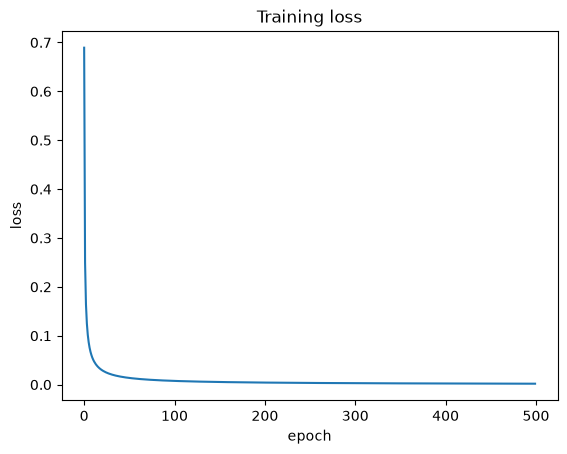
\includegraphics[width=0.5\textwidth]{figures/lesson31_fig04.png}
\caption{Training loss over 500 epochs of gradient descent.}
\label{fig:l31-4}
\end{figure}

\subsection*{Compare to Chapter~\ref{ch:lesson30}'s hand-picked direction}

Normalizing both directions to unit length: the hand-picked direction is $[0.838, 0.546]$, the learned direction is $[0.816, 0.577]$ --- an angle of just $2.2^\circ$ apart. Gradient descent, starting from nothing but random noise, rediscovers essentially the same direction a human picked by reasoning about class means --- reassuring, but also a preview of the limits of a single neuron: it can only ever \emph{rediscover} what a single linear projection is capable of.

\section{Training on the unsolvable problem}

Chapter~\ref{ch:lesson30} showed that \emph{no} linear projection separates a ring from the disk it surrounds --- the best exhaustive search over directions and thresholds found was $74\%$ accuracy. What happens when gradient descent, rather than brute-force search, tries to solve the same problem? Trained for 2000 epochs: the learned weight vector shrinks to near-zero ($\|w\|=0.0824$), and accuracy lands at $50.0\%$ --- chance level, \emph{worse} than the brute-force search's $74\%$.

Gradient descent actually does worse here than brute-force search --- it converges to a near-zero weight vector instead of finding the small, lopsided arc that let a brute-force search eke out $74\%$. The dataset is (approximately) symmetric around the origin, so the \emph{average} gradient pull from all the training points nearly cancels out in every direction, and the optimizer settles near $w\approx0$ rather than hunting for an asymmetric corner-case solution. Different failure mode, same underlying truth: a single linear projection cannot solve this problem, no matter how it's found. Chapter~\ref{ch:lesson32} fixes this --- not by using a smarter optimizer, but by giving the model more than one projection to work with.

\subsection*{Exercises}
\begin{enumerate}
  \item Increase \code{lr} in \code{train} well past a reasonable value (e.g.\ \code{lr=20}) on the two-blob dataset. What happens to the loss curve, and how does this relate to the step size overshooting the loss surface's curvature?
  \item Retrain on the two-blob dataset with several different random seeds. Does the learned direction always end up close to the hand-picked one from Chapter~\ref{ch:lesson30}, or does it vary a lot? What does that suggest about how many good solutions exist for a well-separated dataset?
  \item Make the outer ring asymmetric instead of a full circle (e.g.\ only half the ring). Retrain the single neuron. Does this genuinely broken symmetry noticeably change the final accuracy compared to the $\sim50\%$ chance-level result on the full ring?
\end{enumerate}

\vfill
\fullcode{lesson31}{lesson31_neural_network_fundamentals}
